\section{Evaluation}

\begin{figure}[tb!]
	\begin{center}
		
\includegraphics[width=2in]{noteclose}
	\end{center}
	\caption{Optimal focused noteclose (u=5cm,focus=125,val=812824)}
	\label{f:noteclose}
\end{figure}

\begin{figure}[tb!]
	\begin{center}
		
\includegraphics[width=2in]{notebook}
	\end{center}
	\caption{Optimal focused notebook (u=10cm,focus=80,val=692750)}
	\label{f:notebook}
\end{figure}

\begin{figure}[tb!]
	\begin{center}
		
\includegraphics[width=2in]{notemid}
	\end{center}
	\caption{Optimal focused notemid (u=20cm,focus=125,val=812824)}
	\label{f:notemid}
\end{figure}

\begin{figure}[tb!]
	\begin{center}
		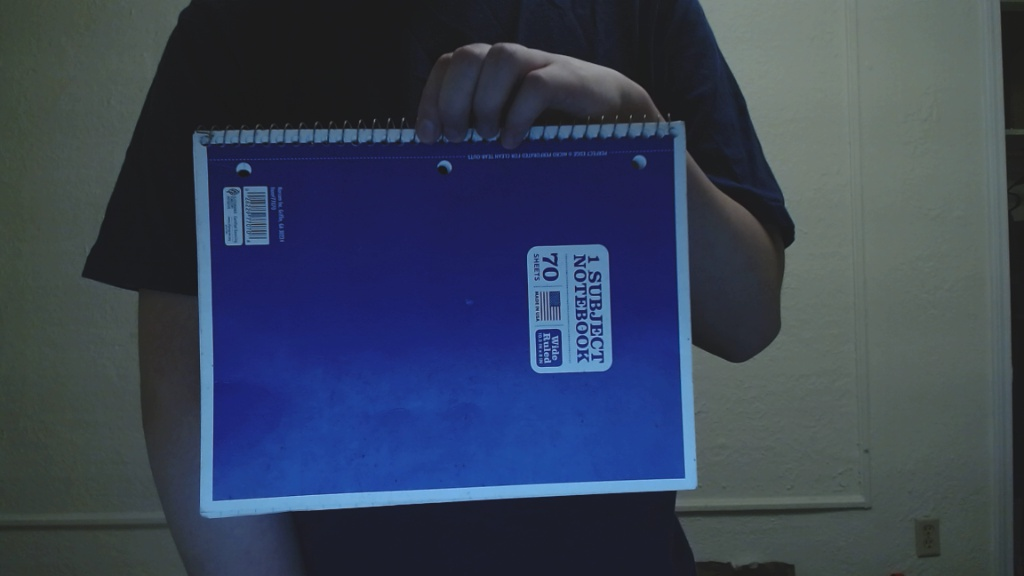
\includegraphics[width=2in]{notefar}
	\end{center}
	\caption{Optimal focused notefar (u=40cm,focus=125,val=812824)}
	\label{f:notefar}
\end{figure}

\begin{figure}[tb!]
	\begin{center}
		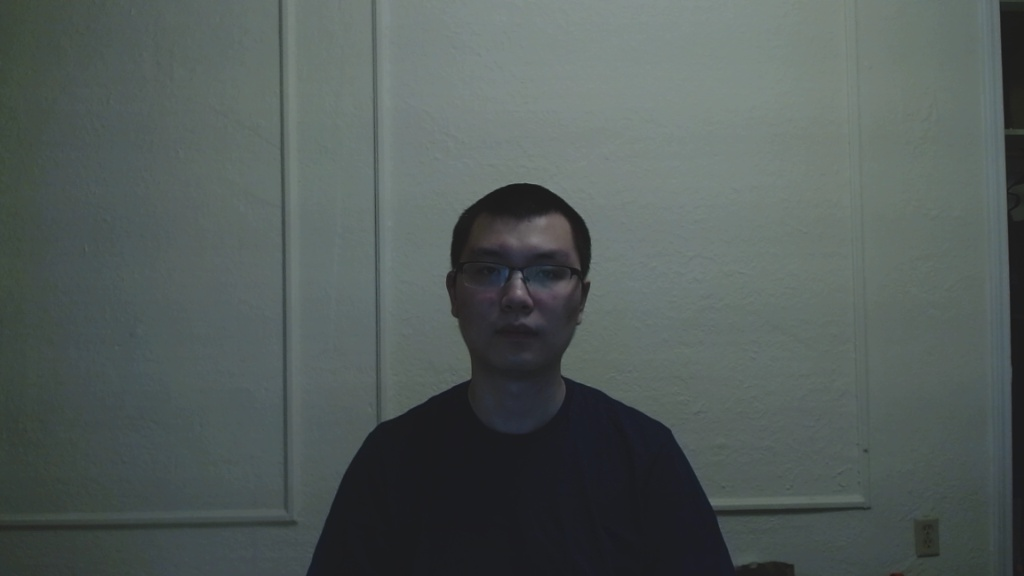
\includegraphics[width=2in]{human}
	\end{center}
	\caption{Optimal focused human (u=1m,focus=125,val=812824)}
	\label{f:human}
\end{figure}

We collect 5 groups of photos, with the object distance from closer to further.
We name the photos as noteclose(Figure~\ref{f:noteclose}), notebook(Figure~\ref{f:notebook}), notemid(Figure~\ref{f:notemid}), notefar(Figure~\ref{f:notefar}), human(Figure~\ref{f:human}) with the distance of 5cm, 10cm, 20cm, 40cm and 1m respectively.
Photos at all focus positions (with 5mm minimum step) are collected in advance and during the evaluation process, the camera is turned on but no photo is collected.
We use the photos collected ahead of time.

\begin{figure}[tb!]
	\begin{center}
		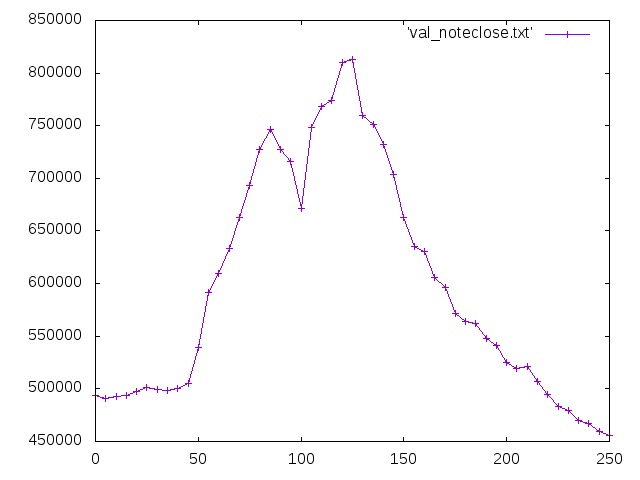
\includegraphics[width=2in]{notecloseplot}
	\end{center}
	\caption{Noteclose: Focus function values under different focus positions}
	\label{f:notecloseplot}
\end{figure}

\begin{figure}[tb!]
	\begin{center}
		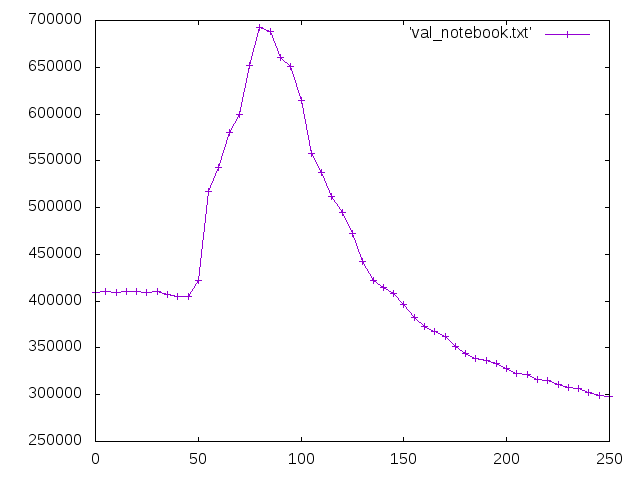
\includegraphics[width=2in]{notebookplot}
	\end{center}
	\caption{Notebook: Focus function values under different focus positions}
	\label{f:notebookplot}
\end{figure}
\begin{figure}[tb!]
	\begin{center}
		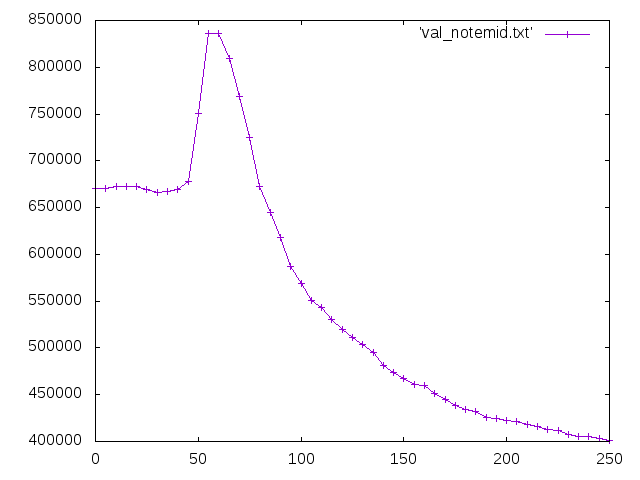
\includegraphics[width=2in]{notemidplot}
	\end{center}
	\caption{Notemid: Focus function values under different focus positions}
	\label{f:notemidplot}
\end{figure}
\begin{figure}[tb!]
	\begin{center}
		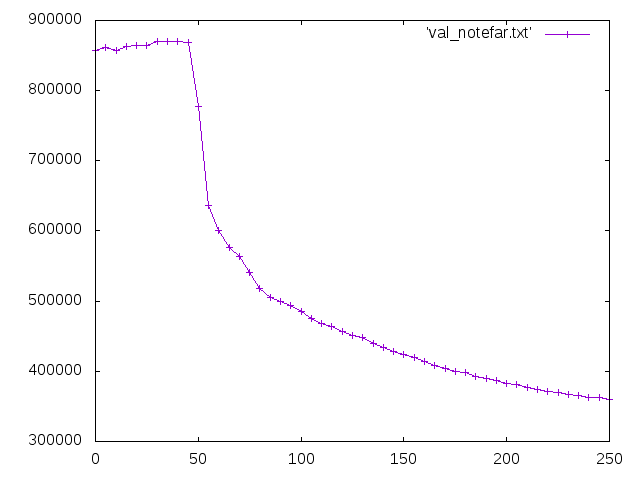
\includegraphics[width=2in]{notefarplot}
	\end{center}
	\caption{Notefar: Focus function values under different focus positions}
	\label{f:notefarplot}
\end{figure}
\begin{figure}[tb!]
	\begin{center}
		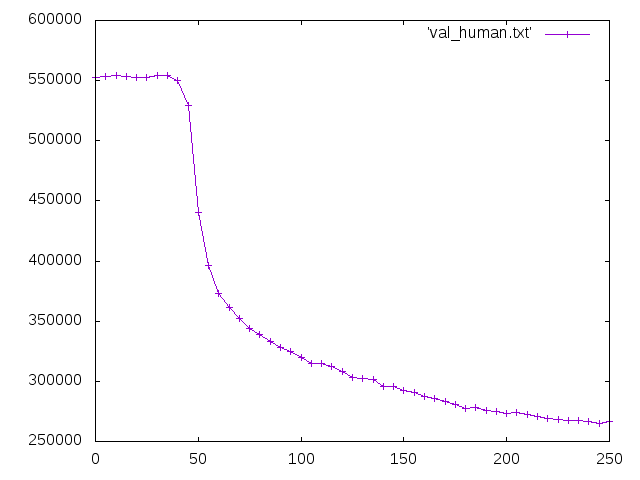
\includegraphics[width=2in]{humanplot}
	\end{center}
	\caption{Human: Focus function values under different focus positions}
	\label{f:humanplot}
\end{figure}

Figure~\ref{f:notecloseplot}, Figure~\ref{f:notebookplot}, Figure~\ref{f:notemidplot}, Figure~\ref{f:notefarplot}, Figure~\ref{f:humanplot} show the focus function values when lens are at different positions.
You may notice that in general, these curves contain only 1 ``hill''.
There are some jitters causing some local maximum appearing.
If there is only 1 ``hill'' in a curve, then the naive hill climbing should be able to reach the global maximum.

\begin{table} [tb!]\tiny
	\centering
	\begin{tabular} {| c | c | c | c | c | c |}
		\hline
		focus/val & \textbf{Noteclose} & \textbf{Notebook} & \textbf{Notemid} & \textbf{Notefar} & \textbf{Human} \\
		\hline
		Optimal(Ground Truth) & 125/812824 & 80/692750 & 60/836247 & 35/870166 & 35/554606 \\
		\hline
		HillClimbing & 85/746181 & 80/692750 & 15/672973 & 5/862217 & 10/554338 \\
		\hline
		\sysname v1 & 125/812824 & 75/652280 & 50/750514 & 25/864501 & 25/552651\\
		\hline
		\sysname v2 & 100/671497 & 100/614299 & 50/750514 & 0/857793 & 0/552585\\
		\hline
	\end{tabular}
	\caption{Focus position and function values of results using different method}
	\label{t:r1}
\end{table}

In Table~\ref{t:r1}, we can see that HillClimbing falls into local maximum in 4 out of 5 cases.
In general, the result function value is not too far away from the ground truth.
But if we combine the results from Table~\ref{t:r2}, we can see that the time of focusing is strongly decided by the number of photos taken.

Next, let us compare v1 and v2 of \sysname.
In Table~\ref{t:r1}, it is obvious that v1 has more accurate results than v2, which means better-focused outcome photos.
However if we take a look at Table~\ref{t:r2}, we can see that the time used by v2 is much shorter than v1, almost halved.
Thus we know that v1 and v2 is a tradeoff between the accuracy and the speed.
\sysname has a more stable focusing time once the step is decided.
Larger step means faster focusing speed and smaller step means better-focused photos.

In Table~\ref{t:r1}, v1 has similar processing time with HillClimbing, but from Table~\ref{t:r1}, surprisingly we see that the focus effect is slightly better than HillClimbing.

\begin{table} [tb!]\scriptsize
	\centering
	\begin{tabular} {| c | c | c | c | c | c |}
		\hline
		Time(s) & \textbf{Noteclose} & \textbf{Notebook} & \textbf{Notemid} & \textbf{Notefar} & \textbf{Human} \\
		\hline
		HillClimbing & 5.71 & 5.07 & 4.29 & 4.16 & 4.69 \\
		\hline
		\sysname v1 & 4.89 & 4.64 & 4.79 & 4.68 & 4.63\\
		\hline
		\sysname v2 & 2.84 & 2.93 & 2.86 & 2.87 & 2.92\\
		\hline
	\end{tabular}
	\caption{Time used on focusing for different groups of photos}
	\label{t:r2}
\end{table}

In Table~\ref{t:r2}, we can see that \sysname v2 greatly speed up the focusing process.
In the best case the speed boost is 50.3\% and on average it is 39.7\% faster.
This is a huge improvement under most cases.

Surely from Table~\ref{t:r1} we can see the quality loss of the picture, in noteclose case it is the worst which is 18\% when evaluated by focus function.
On average, it is a 8.1\$ loss.

To give people a better understanding about the loss, we show you the worst case result provided by \sysname v2 in Figure~\ref{f:worst}.
Compared with Figure!\ref{f:noteclose}, it is not bad at all.

\begin{figure}[tb!]
	\begin{center}
		
\includegraphics[width=2in]{worst}
	\end{center}
	\caption{Worst case blurry for noteclose}
	\label{f:worst}
\end{figure}

